\documentclass[11pt]{article}
\usepackage[UTF8]{ctex}
\usepackage[a4paper]{geometry}
\geometry{left=2.0cm,right=2.0cm,top=2.5cm,bottom=2.5cm}

\usepackage{comment}
\usepackage{booktabs}
\usepackage{graphicx}
\usepackage{diagbox}
\usepackage{amsmath,amsfonts,graphicx,amssymb,bm,amsthm}
%\usepackage{algorithm,algorithmicx}
\usepackage[ruled]{algorithm2e}
\usepackage[noend]{algpseudocode}
\usepackage{fancyhdr}
\usepackage{tikz}
\usepackage{graphicx}
\usetikzlibrary{arrows,automata}
\usepackage{hyperref}
\hypersetup{
	colorlinks=true,
	linkcolor=blue,
	filecolor=blue,      
	urlcolor=blue,
	citecolor=cyan,
}			
\usepackage{listings}
\usepackage{xcolor}

\lstset{
    language=Python,                     % 语言
    basicstyle=\ttfamily,                % 基本字体
    keywordstyle=\bfseries\color{blue},  % 关键字颜色
    commentstyle=\itshape\color{gray},   % 注释颜色
    stringstyle=\color{red},             % 字符串颜色
    showstringspaces=false,              % 不显示字符串中的空格
    frame=single,                        % 添加边框
    breaklines=true                      % 自动换行
}
\setlength{\headheight}{14pt}
\setlength{\parindent}{0 in}
\setlength{\parskip}{0.5 em}

\newtheorem{theorem}{Theorem}
\newtheorem{lemma}[theorem]{Lemma}
\newtheorem{proposition}[theorem]{Proposition}
\newtheorem{claim}[theorem]{Claim}
\newtheorem{corollary}[theorem]{Corollary}
\newtheorem{definition}[theorem]{Definition}
\newtheorem*{definition*}{Definition}

\newenvironment{problem}[2][Problem]{\begin{trivlist}
\item[\hskip \labelsep {\bfseries #1}\hskip \labelsep {\bfseries #2.}]}{\hfill$\blacktriangleleft$\end{trivlist}}
\newenvironment{answer}[1][Answer]{\begin{trivlist}
\item[\hskip \labelsep {\bfseries #1.}\hskip \labelsep]}{\hfill$\lhd$\end{trivlist}}

\newcommand\E{\mathbb{E}}
\newcommand\per{\mathrm{per}}


\title{Homework \#2}
\usetikzlibrary{positioning}

\begin{document}

\pagestyle{fancy}
\lhead{Peking University}
\chead{}
\rhead{Mathematical Foundations for the Information Age, 2024 Fall}

\begin{center}
    {\LARGE \bf Homework \#2}\\
    {Due: 2024-10-21 23:59 \quad$|$\quad 7 Problems, 100 Pts}\\
    {Name: 徐靖, ID: 2200012917}            % Write down your name and ID here.
\end{center}


\begin{problem}{1 (20')} Consider a cube $C$ with side length $1$ in $d$-dimensional space.
\begin{itemize}
    \item [(1)] (4') Write down the radius of a ball $B$ whose volume is equal to the cube's. You don't need to prove your result.
    \item [(2)] (16') When the centers of the cube $C$ and the ball $B$ are both at the origin, calculate the volume of their intersection when $d\to+\infty$.
    \item [] \textit{[Hint: Try to calculate $\mathbb{E}_{X\sim C}[\|X\|_2^2]$ and $Var_{X\sim C}[\|X\|_2^2]$. Then use Chebyshev's Inequality to analyze the concentration of $\|X\|_2^2$. You may use the Stirling's approximation}
    \begin{align*}
        \lim_{n\to+\infty}\frac{\Gamma(n+1)}{\sqrt{2\pi n}(n/\mathrm{e})^n}=1.\tag*{\textit{]}}
    \end{align*}
\end{itemize}
\end{problem}

\begin{answer} ~
\begin{itemize}
    \item [(1)]
Let $r$ donate the radius.
$$r = \pi^{-\frac{1}{2}}\left(\frac{d\Gamma \left(\frac{d}{2}\right)}{2}\right)^{\frac{1}{d}}$$
    \item [(2)]
First we calculate $\mathbb{E}_{X\sim C}[\|X\|_2^2]$ and $Var_{X\sim C}[\|X\|_2^2]$ step by step.
Let $ X_i $ denote the components of $ X $, where $ X \sim C $. Given that $
X_i \stackrel{i.i.d.}{\sim} C, i \in [n] $,we have:
\[
\begin{align*}
\mathbb{E}_{X \sim C}\left[X_i^2\right] &= \int_{-\frac{1}{2}}^{\frac{1}{2}} X_i^2 \, \mathrm{d}X_i = \frac{1}{12} \\
\mathbb{E}_{X \sim C}\left[X_i^4\right] &= \int_{-\frac{1}{2}}^{\frac{1}{2}} X_i^4 \, \mathrm{d}X_i = \frac{1}{80} \\
\mathbb{E}_{X \sim C}\left[\|X\|_2^2\right] &= \sum_{i=1}^d \mathbb{E}_{X \sim C}\left[X_i^2\right] = \frac{d}{12} \\
\mathbb{E}_{X \sim C}\left[\|X\|_2^4\right] &= \mathbb{E}_{X \sim C}\left[\left(\sum_{i=1}^{d-1}X_i^2\right)^2\right] + 2 \mathbb{E}_{X \sim C}\left[X_d^2\right] \cdot \mathbb{E}_{X \sim C}\left[\sum_{i=1}^{d-1}X_i^2\right] + \mathbb{E}_{X \sim C}\left[X_d^4\right]\\
&= \mathbb{E}_{X \sim C}\left[\left(\sum_{i=1}^{d-1}X_i^2\right)^2\right] + \frac{d-1}{72}+\frac{1}{80}\\
&=\sum_{i=1}^d \frac{d-1}{72}+\frac{1}{80} =\frac{d^2}{144}+\frac{d}{180}\\
Var_{X\sim C}[\|X\|_2^2]&=\mathbb{E}_{X \sim C}\left[\|X\|_2^4\right] - \mathbb{E}_{X \sim C}\left[\|X\|_2^2\right]^2 = \frac{d}{180}
\end{align*}
\]
Then we analyze the concentration of $\|X\|_2^2$.
Given that,
$$
\begin{align*}
\mathbb{P}_{X\sim C} [X\in B] &= \mathbb{P}_{X\sim C} \left[\|X\|_2^2<r^2\right]\\
&= \mathbb{P}_{X\sim C} \left[\|X\|_2^2- \mathbb{E}\left[\|X\|_2^2\right]<r^2-\frac{d}{12}\right]\\
&\leq \mathbb{P}_{X\sim C} \left[\left|\|X\|_2^2- \mathbb{E}\left[\|X\|_2^2\right]\right|>|\frac{d}{12}-r^2|\right]\\
&\leq \frac{Var_{X\sim C}[\|X\|_2^2]}{\left(r^2-\frac{d}{12} \right)^2}\\
&=\frac{\frac{d}{180}}{\left(\pi^{-1}\left(\frac{d\Gamma \left(\frac{d}{2}\right)}{2}\right)^{\frac{2}{d}}-\frac{d}{12} \right)^2}\\
&\rightarrow 0 \quad (d \rightarrow +\infty) \quad \text{(using Stirling's approximation)}
\end{align*}
$$
Thus we find that:
$$\lim_{d\rightarrow +\infty} \mathbb{P}_{X\sim C} [X\in B] =0$$
 Hence,
$$V(C\cap B)=0$$
\end{itemize}
\end{answer}



\begin{problem}{2 (16')}
You select a PE class this term, so you need to complete a total of 85km of extracurricular exercise. There are only $n$ days before the deadline, but you still have $m$ kilometers remaining. To simplify your work, you can run at most 10km every day, but there is no lower bound. You are mindless when running, so the distance you run every day is uniformly random. In other words, the number of kilometers you run every day is a real number uniformly selected from range $[0,10]$. Prove that, the probability that you can complete $m$ kilometers in $n$ days, i.e., the probability that your total distance in $n$ days is greater than or equal to $m$ kilometers is 
\begin{align*}
    1-\sum_{i=0}^{\min(\lfloor m/10\rfloor,n)}\frac{(-1)^i}{i!(n-i)!}\left(\frac{m}{10}-i\right)^n.
\end{align*}
\end{problem}
\begin{answer} ~
Let $\{x_i\}$ denote the numbers of kilometers divided by 10 , we have,
$$\underset{x_i\sim U(0,1)}{\mathbb P} (10\sum_{i\in [n]} x_i \ge m)=1-\frac{V(x_i\sim U(0,1),\sum_{i\in [n]} x_i \leq m/10)}{V(x_i\sim U(0,1))}$$ 
Let $U= \{\boldsymbol x|\|\boldsymbol{x}\|_1\leq \frac{m}{10},x_i\ge 0\}$, $A_i=\{\boldsymbol x|\boldsymbol{x}\in U, x_i\leq 1\}$. Naturally, $\overline{A_i}=U\setminus A_i$.
$$V(x_i\sim U(0,1),\sum_{i\in [n]} x_i \leq m/10)=V\left(\bigcap_{i\in [n]}A_i\right)$$
According to the inclusion-exclusion principle,
$$\begin{align*}V\left(\bigcap_{i\in [n]}A_i\right)&=\sum_{k\in [n]}(-1)^{k+1}\sum_{1\leq i_1\leq ...\leq i_k\leq n}V\left(\bigcap_{j\in [k]}A_{i_j}\right)\\&=\sum_{k\in [n]}(-1)^{k+1}\binom{n}{k}\left(V(U)-V\left(\bigcup_{j\in [k]}\overline{A_{i_j}}\right)\right)\\&=\sum_{k\in [n]}(-1)^{k}\binom{n}{k}V\left(\bigcup_{j\in [k]}\overline{A_{i_j}}\right)+V(U)\sum_{k\in [n]}(-1)^{k+1}\binom{n}{k}\end{align*}$$
Note that
$$\sum_{k\in [n]}(-1)^{k+1}\binom{n}{k}=0$$ 
and (The choice of $i_j$ is arbitrary, because $x_i$ is iid.)
$$ V\left(\bigcup_{j\in [k]}\overline{A_{i_j}}\right)=\begin{cases}0,\quad &k\ge m/10\\ \frac{1}{n!}\left(\frac{m}{10}-k\right)^n, &k<m/10\end{cases}$$
Thus, 
$$\begin{align*}V\left(\bigcap_{i\in [n]}A_i\right)&=\sum_{i\in [n] , k<m/10}\frac{(-1)^i}{i!(n-i)!}\left(\frac{m}{10}-i\right)^n\end{align*}$$
which means,
$$\underset{x_i\sim U(0,1)}{\mathbb P} (10\sum_{i\in [n]} x_i \ge m)=1-\sum_{i=0}^{\min(\lfloor m/10\rfloor,n)}\frac{(-1)^i}{i!(n-i)!}\left(\frac{m}{10}-i\right)^n$$

\end{answer}


\begin{problem}{3 (10')}
If $A$ is square, show that $AA^\top$ and $A^\top A$ are similar.

\textit{[Hint: Use the SVD of $A$.]}
\end{problem}
\begin{answer}~
Let \( A \) be an \( n \times n \) matrix. By the Singular Value Decomposition (SVD), we have:

\[
A = U D V^\top
\]

where \( U \) and \( V \) are orthogonal matrices, and \( D \) is a diagonal matrix containing the singular values of \( A \).Then we have:
$$
\begin{align*}
    AA^\top &= A A^\top = (U D V^\top)(U D V^\top)^\top 
        = U D V^\top V D^\top U^\top = U D^2 U^\top \\
    A^\top A &= (U D V^\top)^\top (U D V^\top) 
            = (V D^\top U^\top)(U D V^\top) = V D^2 V^\top
\end{align*}
$$
Let $P=VU^{-1}$, we have:
$$PAA^\top  P^{-1}=VU^{-1}UD^2U^\top UV^{-1}=VD^2V^\top$$
Hence $AA^\top$ and $A^\top A$ are similar.
\end{align*}

\end{answer}


\begin{problem}{4 (12')}
Calculate the SVD of matrix $A$, where 
\begin{align*}
    A=\begin{pmatrix}
        -4&-6\\3&-8
    \end{pmatrix}.
\end{align*} 
You need to calculate it in two different ways.

\textit{[Hint: Use the definition of singular vectors, or consider $A^\top A$.]}
\end{problem}
\begin{answer} ~ \\
\textbf{Method 1}\\
Assume $\boldsymbol v=(x,y)^\top$, then we have $\|A\boldsymbol{v}\|=25x^2+100y^2$
Next, we look for singular vectors one by one.
$$\boldsymbol{v}_1=\underset{|\boldsymbol{v}|=1}{\arg \max} \|A\boldsymbol{v}\|=(0,1)^\top,\sigma_1=\sqrt{\|A\boldsymbol{v_1}\|}=10\\ \boldsymbol{v}_2=\underset{|\boldsymbol{v}|=1,\boldsymbol{v}\bot\boldsymbol{v}_1}{\arg \max}\|A\boldsymbol{v}\|=(1,0)^\top,\sigma_2=\sqrt{\|A\boldsymbol{v_2}\|}=5$$
Then we have,
$$\boldsymbol{u}_1=\frac{A\boldsymbol{v}_1}{\sigma_1}=(-0.6,-0.8)^\top,\boldsymbol{u}_2=\frac{A\boldsymbol{v}_2}{\sigma_2}=(-0.8,0.6)^\top$$
Hence,
$$A=\begin{pmatrix}-0.6&-0.8\\-0.8&0.6\end{pmatrix}\text{diag}\{10,5\}\begin{pmatrix}0&1\\1&0\end{pmatrix}$$
\textbf{Method 2}\\
Consider 
$$A^\top A=\begin{pmatrix}25 & 0\\0 & 100\end{pmatrix}.$$
Solve the equation $|A^\top A-\lambda I|=0$, we get $\lambda=25,100$,
which means $\sigma_1=10,\sigma_2=5$. Then solve equations $(A^TA-\lambda_iI)\boldsymbol{v}=1,|v|=1$ separately, We get the eigenvector $\{v_i\}$ ,then left singular vectors$\{u_i\}$, the solution is obviously same as Method 1.
\end{answer}


\begin{problem}{5 (16')}
Let $A=\sum_{i=1}^{r}\sigma_iu_iv_i^\top$ be the SVD of a rank-$r$ matrix $A$, let $A_k:=\sum_{i=1}^k\sigma_iu_iv_i^\top$ be the rank-$k$ approximation of $A$ for some $k<r$. 
\begin{itemize}
    \item [(1)] (4') Express the following quantities in terms of the singular values $\{\sigma_i,1\le i\le r\}$. You don't need to prove your result.
    \begin{itemize}
        \item [(a)] (2') $\|A_k\|_F^2$.
        \item [(b)] (2') $\|A_k\|_2^2$.
    \end{itemize}
    \item [(2)] (3') Prove that, $\sigma_k\le \frac{\|A\|_F}{\sqrt{k}}$ for $k=1,2,\cdots,r$.
    \item [(3)] (9') Suppose $A\in\mathbb{R}^{m\times m}$. Let $B=\sum_{i=1}^r\frac{1}{\sigma_i}v_iu_i^\top$.  
    \begin{itemize}
        \item [(a)] (6') Show that $BAx=x$ for all $x$ in the span of the right singular vectors of $A$. For this reason $B$ is sometimes called the pseudo inverse of $A$ and can play the role of $A^{-1}$ in many applications.
        \item [(b)] (3') Does $BAx=x$ always hold for all $x\in\mathbb{R}^m$? Prove or give a counterexample.
    \end{itemize}
\end{itemize}
\end{problem}
\begin{answer} ~
\begin{itemize}
    \item [(1)] 
    \begin{itemize}
        \item [(a)] $\|A_k\|_F^2=\sum_{i\in [k]}\sigma_i^2$
        \item [(b)] $\|A_k\|_2^2=\sigma_1^2$
    \end{itemize}
    \item [(2)]              
\\This seems obvious because the singular values are decreasing. And we have shown that the square of the Frobenius norm is equal to the sum of the squares of the singular values.
$$\|A\|_F=\sqrt{\sum_{j\in [n]} |\boldsymbol{a}_j|^2}=\sqrt{\sum_{j\in [n],i\in [r]}(\boldsymbol{a}_j\cdot v_i)^2}=\sqrt{\sum_{i\in [r]}\sigma_i^2(A)}\ge\sqrt{k\sigma_k^2(A)}$$
    \item [(3)]
    \begin{itemize}
        \item [(a)] 
\\Note that
$$\begin{align*}
BA &= \left(\sum_{k=1}^r \frac{1}{\sigma_k}\boldsymbol{v}_k\boldsymbol{u}_k^\top \right)\left(\sum_{k=1}^r \sigma_k \boldsymbol{u}_k\boldsymbol{v}_k^\top \right)\\
&=\sum_{k=1}^r \boldsymbol{v}_k\boldsymbol{u}_k^\top \boldsymbol{u}_k\boldsymbol{v}_k^\top  + \sum_{k=1}^r\sum_{j\in [r]\setminus\{k\}}\boldsymbol{v}_k\boldsymbol{u}_k^\top \boldsymbol{u}_j\boldsymbol{v}_j^\top\\
&=\sum_{k=1}^r \boldsymbol{v}_k\boldsymbol{v}_k^\top
\end{align*}$$
and $\boldsymbol{v}_1,⋯,\boldsymbol{v}_r $ is a basis of the span of the right-singular vectors of $A$. For any $1\leq i\leq r$,
$$BA\boldsymbol{v}_i=\sum_{k=1}^r \boldsymbol{v}_k\boldsymbol{v}_k^\top \boldsymbol{v}_i=\boldsymbol{v}_i$$
thus for any $\boldsymbol{x}$ in the span of the right-singular vectors of $A$,
$$BA\boldsymbol{x}=\boldsymbol{x}$$
        \item [(b)] Not necessarily true. If $A$ is not rank-full, then there exists $x\neq 0$ such that $Ax=0$, then $BAx=0\neq x$. Naturally, when $A$ is full-rank, the set of orthonormal vectors $\{v_i\}$ spans the space $\mathbb{R}^m$, so the conclusion holds.
    \end{itemize}
\end{itemize}
\end{answer}



\begin{problem}{6 (16')}
In class, we introduced the best-fit subspace for a set of points. We extend this definition to probability densities instead of a set of points. If $P$ is a probability density in $\mathbb{R}^d$, then we define the best-fit $k$-dimensional subspace ($k\leq d$)
\begin{align*}
V_k=\arg\max_{V,\mathrm{dim}(V)=k}\E_{X\sim P}(|\mathrm{proj}(X,V)|^2),
\end{align*}
where $\mathrm{proj}(X,V)$ is the orthogonal projection of $X$ onto $V$.
\begin{itemize}
    \item [(1)] (6') Find out the best-fit $1$-dimensional subspace (i.e., a best-fit line through the origin) for probability density $\mathcal{N}\left(0,0,1,2,\frac{1}{2}\right)$.
    \item [] \textit{[Hint: Suppose random variable $(X_1,X_2)\sim\mathcal{N}\left(0,0,1,2,\frac{1}{2}\right)$, then we have}
    \begin{align*}
        X_1\sim\mathcal{N}(0,1),\;X_2\sim\mathcal{N}(0,2),\;\rho:=\frac{\mathbb{E}(X_1X_2)-\mathbb{E}(X_1)\mathbb{E}(X_2)}{\sqrt{Var(X_1)Var(X_2)}}=\frac12.\tag*{\textit{]}}
    \end{align*}
    \item [(2)] (10') Prove that, for $d$-dimensional Gaussian distribution $\mathcal{N}(\mu,I_d)$, a $k$-dimensional subspace is a best-fit subspace if and only if it contains $\mu$.
    \item [] \textit{[Hint: Suppose random variable $(X_1,\cdots,X_d)\sim\mathcal{N}(\mu,I_d)$, then we have $X_i\sim\mathcal{N}(\mu_i,1)$ and $X_1,\cdots,X_d$ are independent random variables.]}
\end{itemize}
\end{problem}
\begin{answer}~
\begin{itemize}
    \item [(1)]Assume unit vector $\boldsymbol{v}_0=(v_1,v_2)^\top$ spans the best-fit 1-dimensional subspace.Then
$$\begin{align*}\boldsymbol{v}_0&=\underset{|\boldsymbol{v}|=1}{\arg 
\max} \underset{X \sim\mathcal{N}\left(0,0,1,2,\frac{1}{2}\right)}{\mathbb E}(|X\cdot \boldsymbol{v}|^2)\\&=\underset{|v|=1}{\arg \max} \;{\mathbb Ea}((X_1v_1+X_2v_2)^2)\\&=\underset{|v|=1}{\arg \max}\; v_1^2+\sqrt{2}v_1v_2+2v_2^2\\&=\left(\sqrt{\frac{3-\sqrt{3}}{6}},\sqrt{\frac{3+\sqrt{3}}{6}}\right)\end{align*}$$ 
Hence the subspace is $\left\{t\boldsymbol{v}_0\big|t\in \mathbb R\right\}$.
    \item [(2)]
Let $\boldsymbol{v}_i$ be a set of standard orthogonal bases of $V$. Note that
$$\begin{align*}\mathbb E_{X\sim \mathcal{N}(\mu_i,I_d)}(|\mathrm{proj}(X,V)|^2)&=\mathbb E_{X\sim \mathcal{N}(\mu_i,I_d)}\left(|\sum_{i\in [k]}(X\cdot\boldsymbol{v}_i)\boldsymbol{v_i}|^2\right)\\&=\mathbb E_{X\sim \mathcal{N}(\mu_i,I_d)}\left(\sum_{i\in [k]}\left(\sum_{j\in [d]}X_jv_{ij}\right)^2\right)\\&=\mathbb E_{X\sim \mathcal{N}(\mu_i,I_d)}\left(\sum_{i\in [k]}\sum_{j\in [d]}X_j^2v_{ij}^2\right)\\&=\sum_{i\in [k]}\sum_{j\in [d]}v_{ij}^2\mathbb E(X_j^2)\\&=\sum_{i\in [k]}\sum_{j\in [d]}v_{ij}^2(\mu_i^2+1)\\&=k+|\mathrm{proj}(\mu,V)|^2\end{align*}$$
That leads to
$$V_k=\underset{V,\mathrm{dim}(V)=k}{\arg\max}|\mathrm{proj}(\mu,V)|^2$$
which means $V_k$ is the subspace that maximizes the projected modulus length of $\mu$ on $V_k$. In other words, it contains $\mu$ (If and only if $\mu$ is within $V_k$, $\mathrm{Proj}(\mu,V)$ reaches the maximum value $|\mu|$)
\end{itemize}
    
\end{answer}


\begin{problem}{7 (10')}
Read in a photochrome and convert to a matrix. Perform a singular value decomposition of the matrix. Reconstruct the photo using only 1,2,4,16 singular values.
\begin{itemize}
    \item [(1)] Print the reconstructed photo. How good is the quality of the reconstructed photo? Write down your observations.
    \item [(2)] What percent of the Frobenius norm is captured in each case? Describe the way you calculate the captured Frobenius norm.
\end{itemize}

You need to include your original photochrome and all reconstructed photos in your answer and submit the code as an attachment.

\textit{[Hint: You may want to perform SVD on each channel.]}
\end{problem}
\newpage
\begin{answer} ~
\begin{itemize}
    \item [(1)] 
    
\begin{figure}[h]
    \centering
    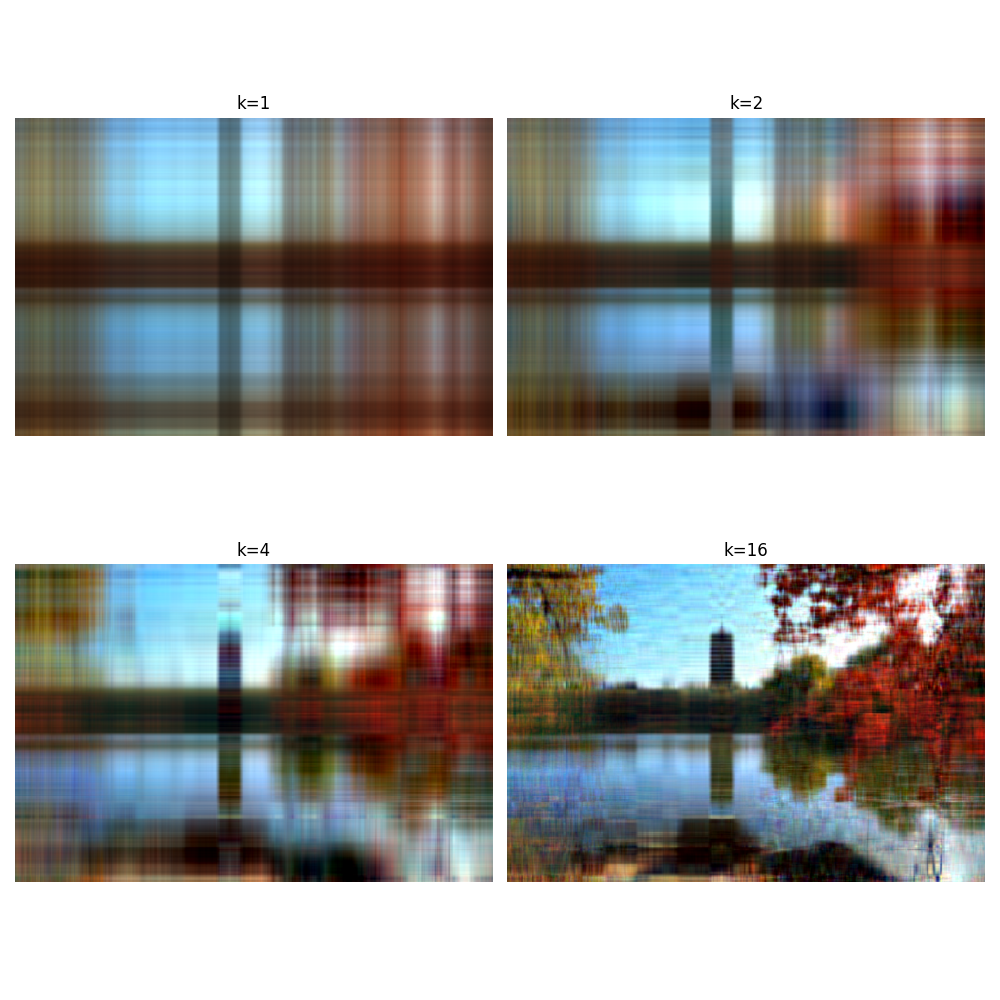
\includegraphics[width=0.6\textwidth]{output1.png} 
    \caption{Rearranged images with different number of singular values $k$}
    \label{fig:sample-image} 

\end{figure}
The image quality increases with the number of singular values. When $k=16$, the image can roughly reflect the characteristics of the original image.
\newpage
    \item [(2)] 

My Frobenius norm calculation is implemented as follows (Python):

\begin{lstlisting}
def frobenius_norm(matrix):
    return np.sqrt(np.sum(matrix ** 2))
\end{lstlisting}

That is, directly calculate the sum of squares of matrix elements.
\begin{table}[!htbp]
    \centering
    \caption{Frobenius norm percentage}
    \begin{tabular}{ccc}
        \toprule
        $k$ & total percentage & percentage of channels \\
        \midrule
        1 & 87.684\% & Channel 0: 89.132\% \\
          &         & Channel 1: 87.982\% \\
          &         & Channel 2: 86.271\% \\
        \hline
        2 & 90.882\% & Channel 0: 91.354\% \\
          &         & Channel 1: 91.317\% \\
          &         & Channel 2: 90.119\% \\
        \hline
        4 & 93.788\% & Channel 0: 93.183\% \\
          &         & Channel 1: 94.147\% \\
          &         & Channel 2: 93.932\% \\
        \hline
        16 & 96.285\% & Channel 0: 95.514\% \\
           &         & Channel 1: 96.433\% \\
           &         & Channel 2: 96.747\% \\
        \bottomrule
    \end{tabular}
    \label{tab:frobenius}
\end{table}
\begin{itemize}
\item My code combines the matrices of the three channels into a three-dimensional matrix and calculates the Frobenius norm together. It is actually equivalent to taking the geometric average of the norms of each channel and then calculating the percentage, which can \textbf{reflect the overall norm change}
\item I once encountered an error of forgetting to do normalization when writing code. Later, I found and solved this bug through another implementation of Frobenius norm:\textbf{ calculating the sum of squares of singular values}. Now the Frobenius norms calculated by the two methods are exactly the same, which shows the correctness of my SVD implementation
\end{itemize}

\end{itemize}
\end{answer}

\end{document}